%!TEX root = ../assignment1.tex

\section{Outcome}
In this section, we gather the findings of two phases of research and seek to invent a general tool for partitioner to evaluate how possible a ICT project is going to succeed.

\subsection{Analysis Of Findings}

\subsubsection{Statistical Analysis}
\paragraph{Average And Standard Deviation}
In Phase 1, the average global influence score is 3.6 and standard deviation
is 2.17. In Phase 2, they are 2.66 and 1.37. It suggests the proposals in Phase 1 has more general influence on how to make ICT project successful. However, standard deviation values indicate the influence power in Phase 1 varies more than that of Phase 2.
\paragraph{Pie Chart By Primary Themes}
To further our analysis on how primary themes(control, process, people and structure) distribute in both Phase 1 and Phase 2, we draw a pie chart to show the proportion.
% \begin{figure}[ht]
% \caption{Primary Themes in Phase 1}
% \centering
% \resizebox{\columnwidth}{!}{%
% 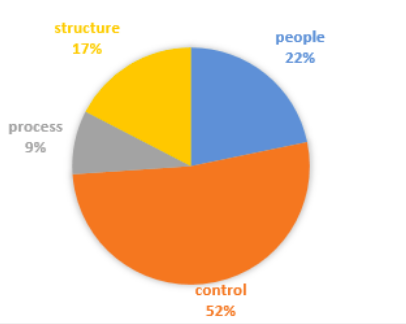
\includegraphics{pie_chart_p1.png}
% }
% \end{figure}

\begin{figure}
\centering
\begin{minipage}{.5\textwidth}
  \centering
  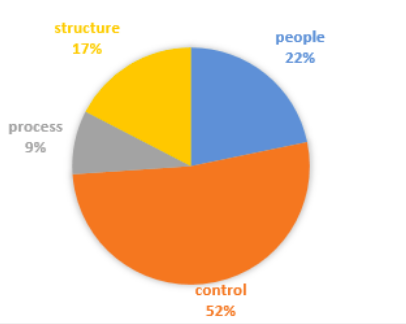
\includegraphics[width=.5\linewidth]{pie_chart_p1.png}
  \captionof{figure}{Primary Themes in Phase 1}
  \label{pie:1}
\end{minipage}%
\begin{minipage}{.5\textwidth}
  \centering
  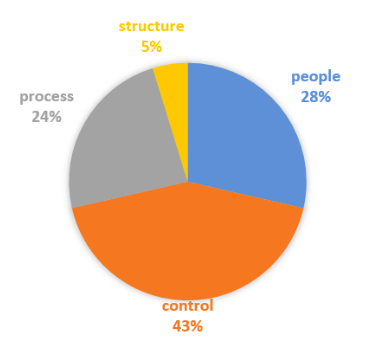
\includegraphics[width=.5\linewidth]{pie_chart_p2.png}
  \captionof{figure}{Primary Themes in Phase 2}
  \label{pie:2}
\end{minipage}
\end{figure}

From the pie charts of \ref{pie:1} and \ref{pie:2}, we can conclude that the theme of control is the dominant theme of solutions followed by the theme of people, which the data of both phases agree to yield. However, there is a subtle difference in the less influential themes of process and structure. Phase 1 puts more emphasis on structure while Phase 2 puts that on process.

\begin{comment}
\section{Comparison}

In this section, a comparison is made to investigate the correlation and the differences of our findings and the Thai business case study. We identify the findings of our sources and our evaluation framework. Correlations are listed as subsection headings.

\subsection{Governance}

In the Thai business case study, the authors argue that risk management can be well developed if both ICT governance and Information security governance
\end{comment}